\documentclass[12pt,a4paper]{report}
\usepackage[utf8]{inputenc}
\usepackage[T1]{fontenc}
\usepackage{xcolor}
\usepackage{graphicx}
\usepackage[french]{babel}
\usepackage{amsmath}
%\usepackage{esint}

\title{ \Huge \textbf{Premier livrable de PlagueINT} \\ \large Modélisation de la propagation des épidémies}
%\date{\today}
\author{
CHERRE Romain
\and COROLLER Stevan 
\and PAMART Pierrick
\and PIPEREAU Yohan
\and \\
Encadrant: Mr. Vincent Gauthier }


\begin{document}
\maketitle

\tableofcontents

\newpage

\addcontentsline{toc}{section}{Analyse des besoins}
\section*{Analyse des besoins}

\addcontentsline{toc}{subsection}{Fonction du produit} %obligé si on utilise pas les numérotations de section et sous section
\subsection*{Fonction du produit}
\begin{flushleft}
  \begin{itemize}
	\item[$\bullet$] Mode de visualisation (écoulement du temps) 
	\item[$\bullet$] Modélisation mondiale avec celulle de la taille d'un pays
	\item[$\bullet$] Possibilité d'exporter le résultat dans un fichier lisible 
	\item[$\bullet$] Voix de transports prise en compte 
	\item[$\bullet$] Possibilité d'ajouter des événements (blocage d'aéroports, gare, etc..) au début
  \end{itemize}
\end{flushleft}

\addcontentsline{toc}{subsection}{Contraintes techniques}
\subsection*{Contraintes techniques}
\begin{flushleft}
  \begin{itemize}
	\item[$\bullet$] Utiliser Java8 avec Eclipse et éventuellement d'autres languages si nécessaires 
	\item[$\bullet$] Possibilité d'execution en mode terminal puis graphique
	\item[$\bullet$] Portabilité Windows, Linux, MAC OS (géré nativement par Java)
    \end{itemize}
\end{flushleft}

\addcontentsline{toc}{subsection}{Critères d'acceptabilité et de réception}
\subsection*{Critères d'acceptabilité et de réception}
\begin{flushleft}
  \begin{itemize}
	\item[$\bullet$] Application performante avec un temps d'exécution raisonnable \\
	\item[$\bullet$] L'interface de l'application doit être conforme à la maquette suivante :\\
\subparagraph*{
------ Simulation de propagation de maladies ------\\
(1) Lancer la simulation\\
(2) Paramètres de simulation\\
(3) Quitter la simulation\\
}
\subparagraph*{  
------ Paramètres de simulation ------\\
(1) Quitter les options sans sauvegarder\\
(2) Date de début et durée de la simulation\\
(3) Pays infectés et nombre d'infectés de départ\\
(4) Choisir les constantes de propagation\\
(5) Gérer les évènements\\
(6) Choisir une maladie pré-enregistrée\\
(7) Quitter et sauvegarder les paramètres\\
}
\subparagraph*{  
------ Evènements ------\\
(1) Créer un évènement\\
(2) Voir les évènements\\
(3) Supprimer un évènement\\
(4) Revenir aux paramètres\\
}
\subparagraph*{  
------ Résultat de la simulation ------\\
(1) Voir la carte du monde\\
(2) Voir les statistiques globales\\
(3) Voir les statistiques d'un pays\\
(4) Extraire le résultat dans un fichier .csv\\
(5) Revenir au menu principal\\
}
  \end{itemize}
\end{flushleft}

\addcontentsline{toc}{subsection}{Extensions}
\subsection*{Extensions}
\begin{flushleft}
  \begin{itemize}
	\item[$\bullet$] Interface - graphique 
	\item[$\bullet$] Informations sur les celulles (petits graphiques, etc...) 
	\item[$\bullet$] Modification de l'environnement (hygiène, température, etc...) 
  \end{itemize}
\end{flushleft}

\addcontentsline{toc}{subsection}{Juridique}
\subsection*{Juridique}
\begin{flushleft}
Creative Commons sans usage commerciale [BY NC SA]
\end{flushleft}

\addcontentsline{toc}{section}{Spécification fonctionnelle générale}
\section*{Spécification fonctionnelle générale}

\addcontentsline{toc}{subsection}{Fonction du produit} %obligé si on utilise pas les numérotations de section et sous section
\subsection*{Fonction du produit}
	\begin{flushleft}
	Pour l'écoulement du temps, nous avons choisi de discrétiser le temps. \\
	Pour l'importation des données et leur traitement, Python est fortement envisagé en tant qu'outil plus performant que Java à l'aide de certaines bibliothèques précodées.
	Pour l'exportation des résultats dans un fichier lisible, on exporterait les données dans un fichier csv en utilisant des fonctionnalités de lecture/écriture de fichier.\\
	Pour modéliser les voix de transports, on utiliserait un seul graphe avec comme noeuds du graphe les pays et sur les branches, le nombre de passagers par jour.
	\end{flushleft}

\addcontentsline{toc}{subsection}{Critères d'acceptabilité et de réception}
\subsection*{Critères d'acceptabilité et de réception}
\begin{flushleft}
	Pour la résolution des équations différentielles, on utiliserait dans un premier temps une méthode d'Euler. Dans un second temps, on implémenterait une méthode de Runge Kutta qui nous permettrait de gagner en performance. \\
	Pour l'interface utilisateur, on permettrait à l'utilisateur de définir l'échelle de temps afin de gérer la rapidité du programme. L'utilisateur pourrait également choisir les pays de lancement de la maladie. Il écrirait le nom du pays et on vérifierait si le nom correspond au nom d'un pays présent dans la liste d'une variable pays. \\
	Enfin pour les coefficients des différentes maladies, il y a le mode manuelle ou l'utilisateur saisi les coefficients à la main et lance ensuite notre programme de modélisation. Mais il y a aussi le mode d'utilisation ou l'utilisateur rentre la maladie et où cela va chercher dans des données que l'on a généré à partir des statistiques mondiales sur les maladies.
\end{flushleft}

\addcontentsline{toc}{subsection}{Extensions}
\subsection*{Extensions}
\begin{flushleft}
 	Pour l'interface graphique qui permettra d'afficher une carte du monde ainsi que de tracer des graphiques relatifs aux données de la celulle et leur évolution dans le temps, nous utiliserons la librairie (toolkit) graphique JavaFX. \\
	Pour la modification de l'environnement (hygiène, température, etc...), on modifie directement les coefficients de propagation de la maladie dans la celulle.
\end{flushleft}

\addcontentsline{toc}{section}{Regroupement modulaire des fonctionnalités}
\section*{Regroupement modulaire des fonctionnalités}
\begin{flushleft}
	\begin{itemize}
		\item[$\bullet$] Visualisation
			\begin{itemize}
				\item Terminal
				\item Graphique
				\item Exportation en CSV
			\end{itemize}
		\item[$\bullet$] Évènements
			\begin{itemize}
				\item Blocage de lieux de transports
				\item Blocage des frontières
			\end{itemize}
		\item[$\bullet$] Statistiques
			\begin{itemize}
				\item Par pays : évolutions du nombre d'infectés, ...
				\item Générales
			\end{itemize}
		\item[$\bullet$] Calcul des évolutions temporelles
	\end{itemize}
\end{flushleft}

\addcontentsline{toc}{section}{Description du flux des données entre les modules}
\section*{Description du flux des données entre les modules}

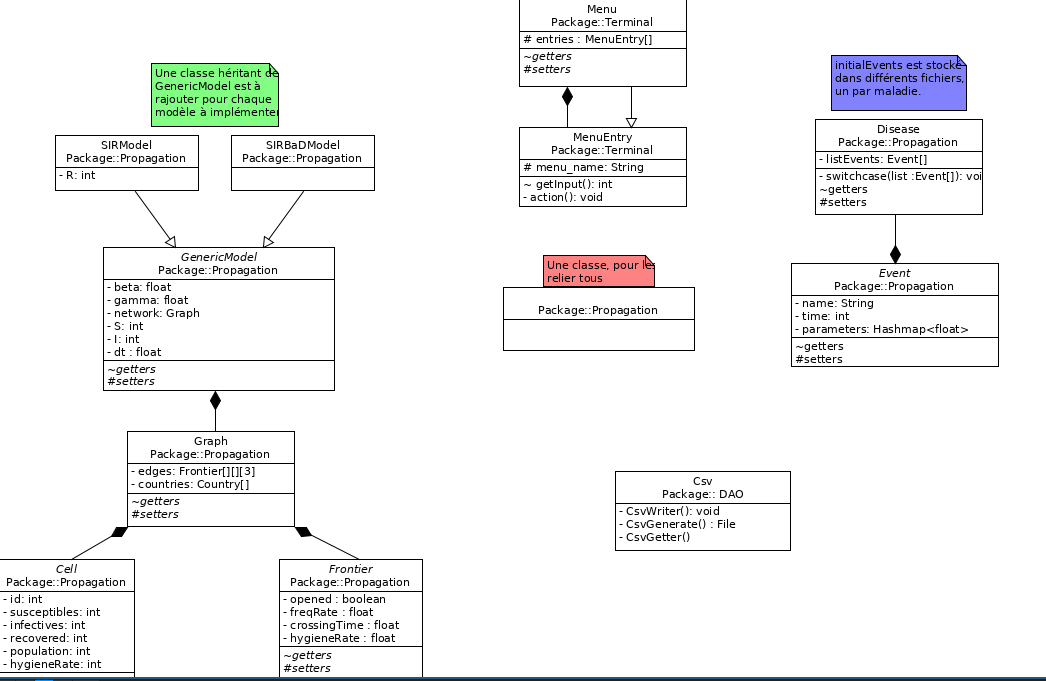
\includegraphics[angle=270 , scale=0.5]{uml.png}

\begin{flushleft}
	Le diagramme UML ci-dessus ne présente pas les relations entre toutes les classes car nous comptons voir comment regrouper certaines classes dans des phases ultérieures de notre développement.
\end{flushleft}
\end{document}
